\documentclass{beamer}
%\usepackage{xspace}
\usepackage{amsmath,amssymb}
\usepackage{graphicx}
%\usepackage{svg}
%\usepackage{pgfpages}
%\pgfpagesuselayout{4 on 1}[a4paper,border shrink=5mm,landscape]
%\usepackage{psfrag}
%\usepackage[usenames,dvipsnames]{xcolor}
\usepackage{braket}
\usepackage{tikz}
\usetikzlibrary{graphs}
\usetikzlibrary{datavisualization}
\usetikzlibrary{datavisualization.formats.functions}
\usepackage{pgfplotstable}
\usepgfplotslibrary{patchplots}

\setbeamercovered{transparent}

\usetheme{Pittsburgh}
%\usetheme{default}

\setbeamertemplate{sidebar right}{}
\setbeamertemplate{footline}[frame number]
%\usefonttheme{professionalfonts}

%\usepackage{sansmathaccent}
%\usepackage{bm}

%\usepackage{unicode-math}
%%\setmainfont[SlantedFont={Latin Modern Roman Slanted},SlantedFeatures={Color=000000},
%%  SmallCapsFont={TeX Gyre Termes},SmallCapsFeatures={Letters=SmallCaps}]{XITS}
%\setmathfont[math-style=ISO,sans-style=upright]{XITS Math}
%\setmathfont[range={\mathcal,\mathbfcal}]{Latin Modern Math}

\usepackage{sfmath}

%\mathversion{sans}

\newcommand{\Tr}{\mathsf{Tr}}

\definecolor{redorange}{rgb}{1.0, .25, .25}
\definecolor{citation}{rgb}{.1, 0.8, .35}
\newcommand\emm[1]{\textcolor{redorange}{{#1}}}
\newcommand\numc[1]{\textcolor{citation}{{\bf #1}}}

%\newcommand\bm[1]{{\mbox{\boldmath $#1$}}}
\newcommand\bm[1]{{\mathbf{#1}}}
%\newcommand\bm[1]{{\bf #1}}
%\newcommand\bm[1]{\ensuremath{\boldsymbol{#1}}}
%\newcommand\bm[1]{{\textbf{\it #1}}}

\title{Introduction to quantum thoery: Quantum states and quantum measurements}
\author{Ryuhei Mori}
%\institute{$\vcenter{\hbox{\includegraphics[width=30pt]{ELC_logo}}}$ Postdoctoral Fellow of ELC\\ $\vcenter{\hbox{\includegraphics[width=20pt]{titech_logo}}}$ Tokyo Institute of Technology}
\institute{Tokyo Institute of Technology}
%\date{21, Feb, 2019}



\begin{document}
\begin{frame}[plain]
\maketitle
\end{frame}


\begin{frame}{What is ``Quantum theory''?}
Quantum theory

\vspace{1em}
\begin{itemize}
\item Physics for microscopic phenomena, e.g., atoms, light.
\end{itemize}

\vspace{2em}
Why is quantum theory important ?

\vspace{1em}
\begin{itemize}
\setlength{\itemsep}{2em}
\item Just because it's reality.
\item Because it gives more efficient information processing, e.g., quantum factoring algorithm, quantum secret-key sharing, etc.
\end{itemize}
\end{frame}

\begin{frame}{On this course}
We study mathematical foundation of quantum information.
\begin{itemize}
\setlength{\itemsep}{1em}
\item Mathematical foundation of quantum physics
\item Quantum algorithms
\item Other quantum information processing, e.g, quantum communication, quantum error-correction.
\end{itemize}

\vspace{2em}
Score
\begin{itemize}
\item Assignments: 70\%
\item Final exam: 30\%
\end{itemize}
\end{frame}

\begin{frame}{Light is wave (1801)}
%\includegraphics[width=0.2\hsize]{young.jpg}
\parbox[b]{0.22\hsize}{\centering\includegraphics[trim={50 120 70 30}, clip,width=1.0\hsize]{Thomas_Young_by_Briggs.jpg}\\ \small Thomas Young\\ (1773 -- 1829)}
\includegraphics[width=0.7\hsize]{Double-slit.pdf}

\centering
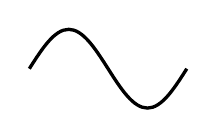
\begin{tikzpicture}[baseline=0]
\draw[black, very thick] (0,0) sin (.5,.5) cos (1,0) sin (1.5,-.5) cos (2,0);
\end{tikzpicture}
\quad $+$ \quad
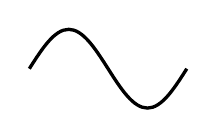
\begin{tikzpicture}[baseline=0]
\draw[black, very thick] (0,0) sin (.5,.5) cos (1,0) sin (1.5,-.5) cos (2,0);
\end{tikzpicture}
\quad $=$ \quad
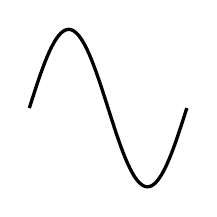
\begin{tikzpicture}[baseline=0]
\draw[black, very thick] (0,0) sin (.5,1) cos (1,0) sin (1.5,-1) cos (2,0);
\end{tikzpicture}

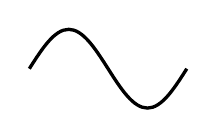
\begin{tikzpicture}[baseline=0]
\draw[black, very thick] (0,0) sin (.5,.5) cos (1,0) sin (1.5,-.5) cos (2,0);
\end{tikzpicture}
\quad $+$ \quad
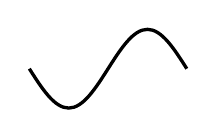
\begin{tikzpicture}[baseline=0]
\draw[black, very thick] (0,0) sin (.5,-.5) cos (1,0) sin (1.5,+.5) cos (2,0);
\end{tikzpicture}
\quad $=$ \quad
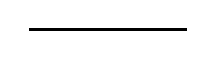
\begin{tikzpicture}[baseline=0]
\draw[black, very thick] (0,0) -- (2,0);
\end{tikzpicture}

\vfill
\scriptsize\url{https://en.wikipedia.org/wiki/Young's_interference_experiment}
\end{frame}

\begin{frame}{Light is particle (1905)}
\centering
\parbox[b]{0.3\hsize}{\centering\includegraphics[clip,width=\hsize]{Einstein_patentoffice.jpg}\\ Albert Einstein\\ (1879 -- 1955)}
\includegraphics[width=0.6\hsize]{Photoelectric_effect.png}

\vfill
\scriptsize\url{https://en.wikipedia.org/wiki/File:Photoelectric_effect.png}
\end{frame}

\begin{frame}{Mach--Zehnder interferometer}
\centering
\begin{tikzpicture}
\draw (0,0) -- (1,0);
\draw[very thick] (0.5,-0.5) -- (1.5,0.5);
\draw[very thick] (5.5,-0.5) -- (6.5,0.5);
\draw[very thick] (0.5,3.5) -- (1.5,4.5);
\draw[very thick] (5.5,3.5) -- (6.5,4.5);
\draw (1,0) -- (6,0) -- (6,4) -- (7,4);
\draw (1,0) -- (1,4) -- (6,4) -- (6,5);
\end{tikzpicture}
\end{frame}

%\begin{frame}{Gravity wave}
%\end{frame}

\begin{frame}{Quantum states and quantum measurements}
\centering
A single photon $\Rightarrow$ BS1 $\Rightarrow$ BS2 $\Rightarrow$ detection

\vspace{2em}
\begin{tabular}{|c|c|}
\hline
State & Measurement \\
\hline
A single photon $\Rightarrow$ BS1 $\Rightarrow$ BS2 & detection\\
A single photon $\Rightarrow$ BS1 & BS2 $\Rightarrow$ detection\\
A single photon & BS1 $\Rightarrow$ BS2 $\Rightarrow$ detection\\
\hline
\end{tabular}

\vspace{5em}
\Large
All understandings are valid
\end{frame}

\begin{frame}{Mathematical representations of states and measurements}
How ``States'' and ``Measurements'' are treated mathematically ?

\vspace{2em}
\centering
A table of probabilities of outcome 'YES' for each binary measurment on each state

\vspace{1em}
\begin{tabular}{|c||c|c|c|}
\hline
& Measurement 1 & Measurement 2 & $\cdots$\\
\hline
\hline
State A& $p_{A1}$ & $p_{A2}$ & $\cdots$\\
State B& $p_{B1}$ & $p_{B2}$ & $\cdots$\\
\vdots& &&\\
\hline
\end{tabular}

\vspace{2em}
* The number of states and measurements are not necessarily countable.

%\textbf{Principle 1}
%
%For any states $A$ and $B$, their probabilistic mixture is also a state.
\end{frame}

\begin{frame}{Classical theory}
States: $\underbar{0}$, $\underbar{1}$

Binary measurements: $\underbar{0}?$, $\underbar{1}?$

\begin{align*}
\underbar{0}?(\underbar{0}) &= 1,&
\underbar{0}?(\underbar{1}) &= 0,\\
\underbar{1}?(\underbar{0}) &= 0,&
\underbar{1}?(\underbar{1}) &= 1
\end{align*}

\begin{center}
\begin{tabular}{|c||c|c|}
\hline
& $\underbar{0}?$& $\underbar{1}?$\\
\hline
\hline
$\underbar{0}$& 1&0\\
\hline
$\underbar{1}$& 0&1\\
\hline
\end{tabular}
\end{center}
\end{frame}


\begin{frame}{State and measurement}
\begin{center}
\begin{tabular}{|c||c|c|}
\hline
& $\underbar{0}?$& $\underbar{1}?$\\
\hline
\hline
$\underbar{0}$& 1&0\\
\hline
$\underbar{1}$& 0&1\\
\hline
\end{tabular}
\end{center}

$S := \text{$\underbar{0}$ with probability $p$,\, $\underbar{1}$ with probability $1-p$}$.

$S$ is also \emm{regarded as a state}.

\begin{align*}
\underbar{0}?(S) &= p,&
\underbar{1}?(S) &= 1-p.
\end{align*}

Similarly,

$E_1 := \text{$\underbar{0}?$ with probability $p$,\, $\underbar{1}?$ with probability $1-p$}$.

$E_2 := \text{$(\underbar{0}\text{ or }\underbar{1})?$}$.

$E_1$ and $E_2$ are also \emm{regarded as a binary measurement}.

\end{frame}

\begin{frame}{Linear space}
\begin{align*}
\omega_{\underbar{0}} &:= \begin{bmatrix}1\\0\end{bmatrix},&
\omega_{\underbar{1}} &:= \begin{bmatrix}0\\1\end{bmatrix}\\
e_{\underbar{0}} &:= \begin{bmatrix}1\\0\end{bmatrix},&
e_{\underbar{1}} &:= \begin{bmatrix}0\\1\end{bmatrix}
\end{align*}
\begin{align*}
{\underbar{0}}?({\underbar{0}}) &= \langle e_{\underbar{0}}, \omega_{\underbar{0}}\rangle,&
{\underbar{0}}?({\underbar{1}}) &= \langle e_{\underbar{0}}, \omega_{\underbar{1}}\rangle\\
{\underbar{1}}?({\underbar{0}}) &= \langle e_{\underbar{1}}, \omega_{\underbar{0}}\rangle,&
{\underbar{1}}?({\underbar{1}}) &= \langle e_{\underbar{1}}, \omega_{\underbar{1}}\rangle
\end{align*}
$S := \text{$\underbar{{\underbar{0}}}$ with probability $p$, $\underbar{{\underbar{1}}}$ with probability $1-p$}$

$\omega_S = p \omega_{\underbar{0}} + (1-p) \omega_{\underbar{1}}=\begin{bmatrix}p\\1-p\end{bmatrix}$.

\vspace{1em}
${\underbar{0}?}(S) = p= \langle e_{\underbar{0}}, \omega_S\rangle$.

\end{frame}

\begin{frame}{States and measurements in a linear space}
\vspace{-1em}
\begin{align*}
\omega_{\underbar{0}} &:= \begin{bmatrix}1\\0\end{bmatrix},&
\omega_{\underbar{1}} &:= \begin{bmatrix}0\\1\end{bmatrix}\\
e_{\underbar{0}} &:= \begin{bmatrix}1\\0\end{bmatrix},&
e_{\underbar{1}} &:= \begin{bmatrix}0\\1\end{bmatrix}
\end{align*}
\begin{equation*}
\text{Set of states} = \left\{\begin{bmatrix}x\\y\end{bmatrix}\mid x\ge 0, y\ge 0, x+y=1\right\}.
\end{equation*}
\begin{equation*}
\text{Set of binary measurements} = \left\{\begin{bmatrix}x\\y\end{bmatrix}\mid x\ge 0, y\ge 0, x\le 1, y\le 1\right\}.
\end{equation*}
\begin{center}
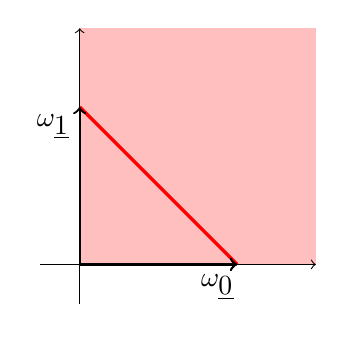
\begin{tikzpicture}
\draw[pink, fill] (0,0) rectangle +(3,3);
\draw[->] (-0.5,0) -- (3,0);
\draw[->] (0,-0.5) -- (0,3);
\draw[very thick, red] (2,0) -- (0,2);
\draw[->, thick] (0,0) -- node[anchor=north, very near end] {$\omega_{\underbar{0}}$} (2,0);
\draw[->, thick] (0,0) -- node[anchor=east, very near end] {$\omega_{\underbar{1}}$} (0,2);
\draw[->, thick] (0,0) -- (2,0);
\end{tikzpicture}
\hfill
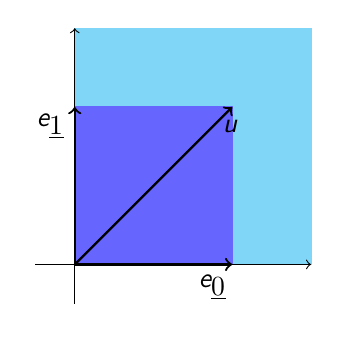
\begin{tikzpicture}
\draw[cyan!50, fill] (0,0) rectangle +(3,3);
\draw[blue!60, fill] (0,0) rectangle +(2,2);
\draw[->] (-0.5,0) -- (3,0);
\draw[->] (0,-0.5) -- (0,3);
%\draw (0,0) -- (2,2);
\draw[->, thick] (0,0) -- node[anchor=north, very near end] {$e_{\underbar{0}}$} (2,0);
\draw[->, thick] (0,0) -- node[anchor=east, very near end] {$e_{\underbar{1}}$} (0,2);
\draw[->, thick] (0,0) -- node[anchor=west, very near end] {$u$} (2,2);
\end{tikzpicture}
\end{center}
\end{frame}

\begin{frame}{State and measurement in a linear space}
\begin{equation*}
\text{Set of states} = \left\{\begin{bmatrix}x\\y\end{bmatrix}\mid x\ge 0, y\ge 0, x+y=1\right\}.
\end{equation*}
\begin{equation*}
\text{Set of binary measurements} = \left\{\begin{bmatrix}x\\y\end{bmatrix}\mid x\ge 0, y\ge 0, x\le 1, y\le 1\right\}.
\end{equation*}
Let $C_{\ge 0}$ be the set of nonnegative vectors and $u:=\begin{bmatrix}1\\1\end{bmatrix}$.
\begin{equation*}
\text{Set of states} = \left\{\omega\in\mathbb{R}^2 \mid \omega\in C_{\ge 0}, \langle u, \omega\rangle = 1\right\}.
\end{equation*}
\begin{equation*}
\text{Set of binary measurements} = \left\{e\in\mathbb{R}^2 \mid e\in C_{\ge 0}, u-e \in C_{\ge 0} \right\}.
\end{equation*}
\begin{align*}
\text{Set of measurements} = \{(e_1,\dotsc,e_k) &\mid e_1+\dotsb+e_k=u,\, e_i\in C_{\ge 0}\\
&\qquad i=1,2,\dotsc,k,\,k=1,2,\dotsc \}
\end{align*}
Outcome of the measurement $M=(e_1,\dotsc,e_k)$ on $\omega$ is $i$ with probability \emm{$\langle e_i, \omega\rangle$}.
\end{frame}


\begin{frame}{Quantum theory}

{\small
$C_{\ge 0}\subseteq\mathbb{R}^2:$ the set of nonnegative vectors, $u:=\begin{bmatrix}1\\1\end{bmatrix}$.
\begin{equation*}
\text{Set of states} = \left\{\omega\in\mathbb{R}^2 \mid \omega\in C_{\ge 0}, \langle u, \omega\rangle = 1\right\}.
\end{equation*}
\begin{equation*}
\text{Set of binary measurements} = \left\{e\in\mathbb{R}^2 \mid e\in C_{\ge 0}, u-e \in C_{\ge 0} \right\}.
\end{equation*}
\begin{align*}
\text{Set of measurements} = \{(e_1,\dotsc,e_k) &\mid e_1+\dotsb+e_k=u,\, e_i\in C_{\ge 0}\\
&\qquad i=1,2,\dotsc,k,\, k=1,2,\dotsc,\}
\end{align*}
}

\vspace{.1em}
$V:$ the linear space on $\mathbb{R}$ spanned by $2\times 2$ Hermitian matrices.\\
$\langle e,\omega\rangle:=\Tr(e\omega)$ for $\omega, e\in V$ (Hilbert-Schmidt inner product).\\
$\emm{C_{\succeq 0}}\subseteq V:$ the set of positive semidefinite matrices, $u:=\begin{bmatrix}1&0\\0&1\end{bmatrix}$.
\begin{equation*}
\text{Set of states} = \left\{\omega\in V \mid \omega\in \emm{C_{\succeq 0}}, \langle u,\omega\rangle = 1\right\}.
\end{equation*}
\begin{equation*}
\text{Set of binary measurements} = \left\{e\in V \mid e\in \emm{C_{\succeq 0}}, u-e \in \emm{C_{\succeq 0}} \right\}.
\end{equation*}
\end{frame}

\begin{frame}{Linear space spanned by 2x2 Hermitian matrices}
Basis
\begin{equation*}
A:=
\begin{bmatrix}
1&0\\
0&0
\end{bmatrix}
,
B:=
\begin{bmatrix}
0&0\\
0&1
\end{bmatrix}
,
C:=
\begin{bmatrix}
0&1\\
1&0
\end{bmatrix}
,
D:=
\begin{bmatrix}
0&-i\\
i&0
\end{bmatrix}
\end{equation*}
Another choice of basis
\begin{equation*}
I:=
\begin{bmatrix}
1&0\\
0&1
\end{bmatrix}
,
X:=
\begin{bmatrix}
0&1\\
1&0
\end{bmatrix}
,
Y:=
\begin{bmatrix}
0&-i\\
i&0
\end{bmatrix}
,
Z:=
\begin{bmatrix}
1&0\\
0&-1
\end{bmatrix}
\end{equation*}

Both are orthogonal basis.

The second basis ($I$ and Pauli matrices $X$, $Y$ and $Z$) has nice properties.
\begin{enumerate}
\item $\Tr(I)=2$. $\Tr(X)=\Tr(Y)=\Tr(Z)=0$.
\item $X^2 = Y^2 = Z^2 = I$ ($X$, $Y$ and $Z$ have eigenvalues $\pm 1$).
\item $XY=-YX,\,YZ=-ZY,\,ZX=-XZ$.
\end{enumerate}
\end{frame}

\begin{frame}{Positive semidefinite cone}
\begin{equation*}
I:=
\begin{bmatrix}
1&0\\
0&1
\end{bmatrix}
,
X:=
\begin{bmatrix}
0&1\\
1&0
\end{bmatrix}
,
Y:=
\begin{bmatrix}
0&-i\\
i&0
\end{bmatrix}
,
Z:=
\begin{bmatrix}
1&0\\
0&-1
\end{bmatrix}
\end{equation*}
\begin{equation*}
\rho = \frac1{\sqrt{2}}\left(a_I I + a_X X + a_Y Y + a_Z Z\right)
\end{equation*}
\begin{align*}
\lambda_1\ge 0,\, \lambda_2\ge 0 &\iff
\lambda_1 + \lambda_2 \ge 0,\, \lambda_1 \lambda_2 \ge 0\\
&\iff \Tr(\rho)\ge 0,\, \Tr(\rho)^2-\Tr(\rho^2)\ge 0\\
&\iff a_I \ge 0,\,  2 a_I^2 - (a_I^2 + a_X^2 + a_Y^2 + a_Z^2) \ge 0\\
&\iff \emm{a_I \ge 0,\,  a_I^2 \ge a_X^2 + a_Y^2 + a_Z^2}
\end{align*}
\begin{equation*}
\Tr(\rho)=1
\iff
a_I=\frac1{\sqrt{2}}
\end{equation*}
\end{frame}

\begin{frame}{Geometry of quantum states and effects}
\begin{tikzpicture}
    \begin{axis}[height= 0.55\vsize, axis lines=center, axis on top, xmin=-1.0, xmax=1.0, ymin=-1.0, ymax=1.0, z buffer = sort, xtick = \empty, ytick=\empty, ztick=\empty ]
    \addplot3[surf, samples= 10, samples y=10, domain= 0:1/sqrt(2), domain y= 0:2*pi, colormap = {pinkpink}{color=(pink) color=(pink)}]
      ({x*cos(deg(y))}, {x*sin(deg(y))}, {x});
    \addplot3[surf, samples= 10, samples y=10, domain= 0:1/sqrt(2), domain y= 0:2*pi, color = red ]
      ({x*cos(deg(y))}, {x*sin(deg(y))}, {1/sqrt(2)});
    \end{axis}
\end{tikzpicture}
\begin{tikzpicture}
    \begin{axis}[height=0.70\vsize, axis lines=center, axis on top, xmin=-1.0, xmax=1.0, ymin=-1.0, ymax=1.0, z buffer = sort, xtick = \empty, ytick=\empty, ztick=\empty ]
    \addplot3[surf, samples= 40, samples y=10, domain= 0:sqrt(2), domain y= 0:2*pi, mesh/interior colormap = {blueblack}{color=(cyan!50) color=(cyan!50)}, colormap = {blueblack}{color=(blue!60) color=(blue!60)}]
      ({(sqrt(2)/2-abs(sqrt(2)/2-x))*cos(deg(y))}, {(sqrt(2)/2-abs(sqrt(2)/2-x))*sin(deg(y))}, {x});
    \end{axis}
\end{tikzpicture}
\end{frame}


\begin{frame}{Convex cone and dual cone}
\begin{align*}
\text{$C\subseteq V$ is a convex cone} \Longleftrightarrow&
\,x+y\in C,\, \lambda x \in C,\\
&\forall x\in C, y\in C,\, \lambda \ge 0
\end{align*}

Proper cone: closed, not $V$, full-dimensional.

\begin{align*}
&\text{$C^*\subseteq V$ is a dual cone of $C$} \\
&\Longleftrightarrow C^*:= \{x\in V\mid \langle x,y\rangle \ge 0,\, \forall y\in C\}
\end{align*}

$C_{\ge 0}$ and $C_{\succeq 0}$ are self-dual cones.
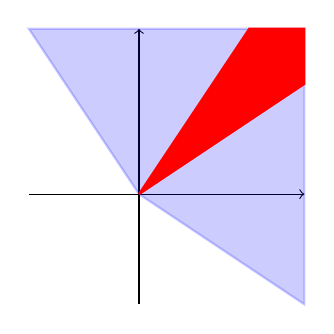
\begin{tikzpicture}[baseline=0,scale=0.7]
%\draw[pink, fill] (0,0) rectangle +(3,3);
\draw[->] (-2,0) -- (3,0);
\draw[->] (0,-2) -- (0,3);
\draw[fill,blue,thick,opacity=0.2] (0,0) -- (-2,3) -- (3,3) -- (3,-2) -- (0,0);
\draw[fill,red,thick] (0,0) -- (3,2) -- (3,3) -- (2,3) -- (0,0);
\end{tikzpicture}

\end{frame}

\begin{frame}{Generalized probabilistic theories}
$\emm{C}:$ convex cone.

$u\in\text{interior of } \emm{C}^*$.

\begin{equation*}
\text{Set of states} = \left\{\omega\in V \mid \omega\in \emm{C}, \langle u,\omega\rangle = 1\right\}.
\end{equation*}
\begin{equation*}
\text{Set of effects} = \left\{e\in V \mid e\in \emm{C}^*, u-e \in \emm{C}^* \right\}.
\end{equation*}
\begin{equation*}
\text{Set of measurements} = \{(e_1,\dotsc,e_k) \mid e_1+\dotsb+e_k=u,\, k=1,2,3,\dotsc\}
\end{equation*}

\vspace{3em}
Classical theory\\
 $V=\mathbb{R}^n,\, C = C_{\ge 0},\, u=\text{the all-1 vector}$.

\vspace{1em}
Quantum theory\\
 $V=\text{A set of $n\times n$ Hermitian matrices},\,C = C_{\succeq 0},\, u=I$.

\vspace{1em}
Other theories ?
%\vspace{1em}
%\begin{center}
%\Large
%What determines the quantum physics?
%
%\vspace{1em}
%\large
%Postulates: no-signaling, tomographic locality, continuous reversibility, $\dotsc,$
%\end{center}
\end{frame}


\begin{frame}{Toy theory: Gbit}
\begin{tikzpicture}
    \begin{axis}[view={20}{20}, height= 0.55\vsize, axis lines=center, axis on top, xmin=-1.0, xmax=1.0, ymin=-1.0, ymax=1.0]
    \addplot3[ colormap={pinkred}{color=(pink) color=(red)}, opacity = 0.9, faceted color = black!80, table/row sep=\\, patch, patch type=polygon, vertex count= 4,
    patch table with point meta = {%
      0 0 1 2 -0\\
      0 0 2 3 -0\\
      0 0 3 4 -0\\
      0 0 4 1 -0\\
      1 2 3 4 10\\
    } ]
      table {
      x y z\\
      0 0 0\\
      0 1 1\\
      1 0 1\\
      0 -1 1\\
      -1 0 1\\
    };
    \end{axis}
\end{tikzpicture}
\hfill
\begin{tikzpicture}
    \begin{axis}[view={20}{10}, height= 0.55\vsize, axis lines=center, axis on top, xmin=-0.5, xmax=0.5, ymin=-0.5, ymax=0.5]
    \addplot3[ colormap={blueblue}{color=(blue!60) color=(blue!60)}, opacity = 0.8, faceted color = black!80, table/row sep=\\, patch, patch type=triangle,
    patch table = {%
      0 1 2\\
      0 2 3\\
      0 3 4\\
      0 4 1\\
      5 1 2\\
      5 2 3\\
      5 3 4\\
      5 4 1\\
    } ]
      table {
      x y z\\
      0 0 0\\
      -0.5 -0.5 0.5\\
      -0.5 0.5 0.5\\
      0.5 0.5 0.5\\
      0.5 -0.5 0.5\\
      0 0 1\\
    };
    \end{axis}
\end{tikzpicture}

\vspace{-1em}
\begin{align*}
\omega_0&=\begin{bmatrix} 1& 0& 1\end{bmatrix},&
\omega_1&=\begin{bmatrix} 0& 1& 1\end{bmatrix},\\
\omega_2&=\begin{bmatrix} -1& 0& 1\end{bmatrix},&
\omega_3&=\begin{bmatrix} 0& -1& 1\end{bmatrix}.
\end{align*}

\vspace{-1em}
\begin{align*}
e_0&=\frac12\begin{bmatrix} 1& 1& 1\end{bmatrix},&
e_1&=\frac12\begin{bmatrix} -1& 1& 1\end{bmatrix},\\
e_2&=\frac12\begin{bmatrix} 1& -1& 1\end{bmatrix},&
e_3&=\frac12\begin{bmatrix} -1& -1& 1\end{bmatrix},\\
u&=\begin{bmatrix} 0& 0& 1\end{bmatrix}.
\end{align*}
\end{frame}

\begin{frame}{Nonlocality}
\centering
OK, generalized probabilistic theory is quite simple and easy to understand.

\vspace{2em}
But, what is essential difference between classical theory and quantum theory ?

\vspace{2em}
Can quantum theory be ``simulated'' or ``explained'' by classical theory ?

\vspace{2em}
Are Hermitian positive-semidefinite matrices really needed for explaining reality ?
\end{frame}

%\begin{frame}{EPR paradox}
%\end{frame}

\begin{frame}{Bell test: CHSH game (1964, 1969)}
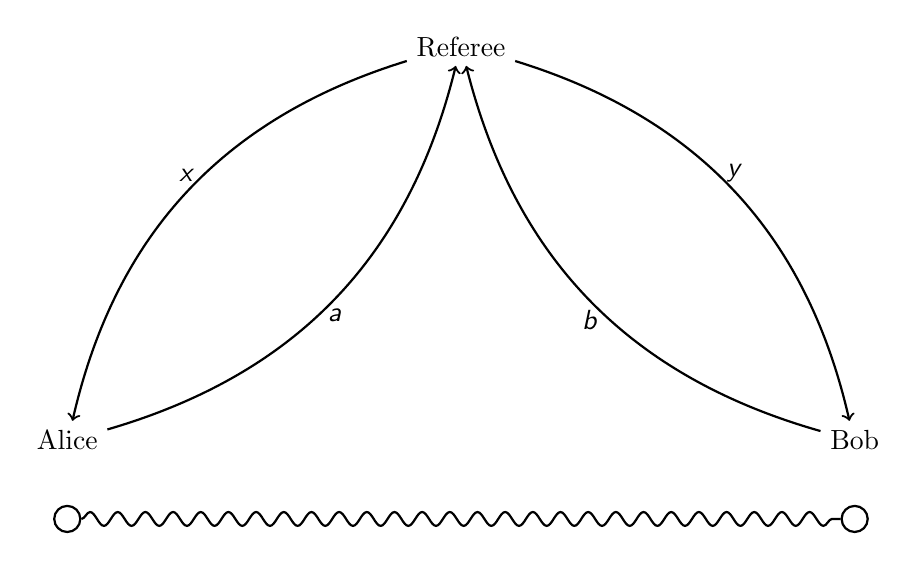
\begin{tikzpicture}
\node at (5,5) (R) {Referee};
\node at (0,0) (A) {Alice};
\node at (10,0) (B) {Bob};
\node at (0,-1)[circle,thick,draw] (As) {};
\node at (10,-1)[circle,thick,draw] (Bs) {};
\draw[->,thick] (R) edge[bend right] node[anchor=south, midway]{$x$} (A);
\draw[->,thick] (R) edge[bend left] node[anchor=south, midway]{$y$} (B);
\draw[->,thick] (A) edge[bend right] node[anchor=north, midway]{$a$} (R);
\draw[->,thick] (B) edge[bend left] node[anchor=north, midway]{$b$} (R);
\draw[thick,decorate,decoration=snake] (As) -- (Bs);
\end{tikzpicture}
%\includegraphics[width=30pt]{Alice_in_Wonderland.png}
\begin{center}
Alice and Bob win iff $\emm{a\oplus b = x\wedge y}$.
\end{center}
\end{frame}

\begin{frame}{Bell inequality}
$a_x$: Output of Alice for given $x$.

$b_y$: Output of Bbob for given $y$.
\begin{align*}
a_0 \oplus b_0 &= 0\\
a_1 \oplus b_0 &= 0\\
a_0 \oplus b_1 &= 0\\
a_1 \oplus b_1 &= 1
\end{align*}
By adding all equations, we get $0=1$, which means there is no solution.
Hence, the winning probability 1 cannot be achieved.

\vspace{1em}
Three equalities can be satisfied, so that the largest winning probability is \emm{3/4}~(Bell inequality or CHSH inequality).

\vspace{1em}
If Alice and Bob share quantum states, then the largest winning probability is
$(2+\sqrt{2})/4\approx \emm{0.854}$~(Violation of Bell/CHSH inequality)
\end{frame}

\begin{frame}{Locality (Hidden variable model)}
\begin{center}
Joint preparation and independent measurements.
\end{center}
Probability distribution $P(a,b\mid x,y)$ is said to be \textbf{local} if
\begin{equation*}
P(a, b\mid x,y) = \sum_{\lambda} P(\lambda) P(a\mid x, \lambda) P(b\mid y,\lambda).
\end{equation*}
\vspace{2em}
\begin{center}
Quantum physics allow \emm{nonlocal} behaviors.
\end{center}
\end{frame}

\begin{frame}{Einstein--Podolsky--Rosen (EPR) paradox (1935)}
\begin{equation*}
P(a, b\mid x,y) = \sum_{\lambda} P(\lambda) P(a\mid x, \lambda) P(b\mid y,\lambda).
\end{equation*}
$\iff$
there exists a joint distribution of $(a_0,a_1,b_0,b_1)$.

\begin{center}
\Large
$\Downarrow$

\vspace{1.0em}
\normalsize
In quantum physics,
$a_0,a_1,b_0,b_1$ \emm{cannot \textit{exists}} simultaneously.

\vspace{1.0em}
\Large
$\Downarrow$

\vspace{1.0em}
\normalsize
In quantum physics,
position and momentum \emm{cannot \textit{exists}} simultaneously.
\end{center}

%[Einstein, Podolsky, Rosen 1935, \numc{15771}]
\end{frame}



\begin{frame}{Summary}
\begin{itemize}
\item .
\item Classical theory and quantum theory are special cases of generalized probabilistic theories.
\end{itemize}



\begin{itemize}
\item Joint system, e.g., two qubits.
\end{itemize}
\end{frame}

\begin{frame}{Assignments}
\begin{enumerate}
\setlength{\itemsep}{2em}
\item Show the dimension and one of the basis of real linear space spanned by $n\times n$ Hermitian matrices
\item Show that $XY=-YX$, $YZ=-ZY$ and $ZX=-XZ$.
\item Show that the Hilbert--Schmidt inner product satisfies the axioms of inner product.
\item Show that $C_{\succeq 0}$ is a self-dual cone.
\end{enumerate}
\end{frame}

\end{document}
